% \documentclass[11pt]{article}
\documentclass[useAMS,usenatbib,referee]{biom}
% \usepackage{amssymb, amsthm, amsmath}
\usepackage{amssymb, amsmath}
\usepackage{bm}
\usepackage{graphicx}
% \usepackage[authoryear]{natbib}
\usepackage{natbib}
\usepackage{bm}
\usepackage{verbatim}
\usepackage{lineno}
\usepackage{times}
\usepackage{soul}
\usepackage{color}
\usepackage{enumitem}
\usepackage{setspace}

% cross-referencing appendices
\usepackage{xr}
\externaldocument{supplemental}

% \usepackage[left=1in,top=1in,right=1in]{geometry}
% \pdfpageheight 11in
% \pdfpagewidth 8.5in
% \linespread{2.0}
\newcommand{\btheta}{ \mbox{\boldmath $\theta$}}
\newcommand{\bmu}{ \mbox{\boldmath $\mu$}}
\newcommand{\balpha}{ \mbox{\boldmath $\alpha$}}
\newcommand{\bbeta}{ \mbox{\boldmath $\beta$}}
\newcommand{\bdelta}{ \mbox{\boldmath $\delta$}}
\newcommand{\blambda}{ \mbox{\boldmath $\lambda$}}
\newcommand{\bgamma}{ \mbox{\boldmath $\gamma$}}
\newcommand{\brho}{ \mbox{\boldmath $\rho$}}
\newcommand{\bpsi}{ \mbox{\boldmath $\psi$}}
\newcommand{\bepsilon}{ \mbox{\boldmath $\epsilon$}}
\newcommand{\bomega}{ \mbox{\boldmath $\omega$}}
\newcommand{\bOmega}{ \mbox{\boldmath $\Omega$}}
\newcommand{\bDelta}{ \mbox{\boldmath $\Delta$}}
\newcommand{\bSigma}{ \mbox{\boldmath $\Sigma$}}
\newcommand{\bPsi}{\mbox{\boldmath $\Psi$}}
\newcommand{\bOne}{\mbox{\boldmath $1$}}
\newcommand{\omu}{\overline{\mu}}
\newcommand{\oSigma}{\overline{\Sigma}}
\newcommand{\Yt}{{\tilde Y}}
\newcommand{\bA}{ \mbox{\bf A}}
\newcommand{\bP}{ \mbox{\bf P}}
\newcommand{\bx}{ \mbox{\bf x}}
\newcommand{\bX}{ \mbox{\bf X}}
\newcommand{\bB}{ \mbox{\bf B}}
\newcommand{\bZ}{ \mbox{\bf Z}}
\newcommand{\by}{ \mbox{\bf y}}
\newcommand{\bY}{ \mbox{\bf Y}}
\newcommand{\bz}{ \mbox{\bf z}}
\newcommand{\bh}{ \mbox{\bf h}}
\newcommand{\br}{ \mbox{\bf r}}
\newcommand{\bt}{ \mbox{\bf t}}
\newcommand{\bs}{ \mbox{\bf s}}
\newcommand{\bb}{ \mbox{\bf b}}
\newcommand{\bL}{ \mbox{\bf L}}
\newcommand{\bu}{ \mbox{\bf u}}
\newcommand{\bv}{ \mbox{\bf v}}
\newcommand{\bV}{ \mbox{\bf V}}
\newcommand{\bW}{ \mbox{\bf W}}
\newcommand{\bG}{ \mbox{\bf G}}
\newcommand{\bH}{ \mbox{\bf H}}
\newcommand{\bw}{ \mbox{\bf w}}
\newcommand{\bo}{ \mbox{\bf o}}
\newcommand{\bfe}{ \mbox{\bf e}}
\newcommand{\iid}{\stackrel{iid}{\sim}}
\newcommand{\indep}{\stackrel{indep}{\sim}}
\newcommand{\calR}{{\cal R}}
\newcommand{\calG}{{\cal G}}
\newcommand{\calD}{{\cal D}}
\newcommand{\calS}{{\cal S}}
\newcommand{\calB}{{\cal B}}
\newcommand{\calA}{{\cal A}}
\newcommand{\calT}{{\cal T}}
\newcommand{\calO}{{\cal O}}
\newcommand{\argmax}{{\mathop{\rm arg\, max}}}
\newcommand{\argmin}{{\mathop{\rm arg\, min}}}
\newcommand{\Frechet}{\mbox{Fr$\acute{\mbox{e}}$chet }}
\newcommand{\Matern}{\mbox{Mat$\acute{\mbox{e}}$rn }}
\newcommand{\ballunion}{B_a(\bs_1) \cup B_b(\bs_2) }

\newcommand{\beq}{ \begin{equation}}
\newcommand{\eeq}{ \end{equation}}
\newcommand{\beqn}{ \begin{eqnarray}}
\newcommand{\eeqn}{ \end{eqnarray}}

\title[A Space-time Skew-$t$ Model for Threshold Exceedances]{A space-time skew-$t$ model for threshold exceedances}
\author
{Samuel A Morris$^{1,*}$\email{samorris@ncsu.edu},
Brian J Reich$^{1}$,
Emeric Thibaud$^{2}$, and
Daniel Cooley$^{2}$\\
$^{1}$Department of Statistics, North Carolina State University, Raleigh, North Carolina, U.S.A. \\
$^{2}$Department of Statistics, Colorado State University, Fort Collins, Colorado, U.S.A.}

\begin{document} %\linenumbers
% \begin{center}
% {\Large {\bf A space-time skew-$t$ model for threshold exceedances}}\\

% {\large Samuel A Morris\footnote[1]{North Carolina State University}, Brian J Reich\footnotemark[1]{}, Emeric Thibaud\footnote[2]{Colorado State University}, and Daniel Cooley\footnotemark[2]{}}

% \today
% \end{center}

\pagerange{\pageref{firstpage}--\pageref{lastpage}}

\label{firstpage}

\begin{abstract}
To assess the compliance of air quality regulations, the Environmental Protection Agency (EPA) must know if a site exceeds a pre-specified threshold.
In the case of ozone, the threshold for compliance is fixed at 75 parts per billion, which is high, but not extreme at all locations.
We present a new method based on the spatial skew-$t$ process.
Our method incorporates a random partition to permit long-distance asymptotic independence while allowing for sites that are near one another to be asymptotically dependent, and we incorporate thresholding to allow the tails of the data to speak for themselves.
We also introduce a transformed AR(1) time-series to allow for temporal dependence.
Finally, our model allows for high-dimensional Bayesian inference that is comparable in speed to traditional geostatistical methods for large datasets.
We apply our method to an ozone analysis for July 2005, and find that our model improves over both Gaussian and max-stable methods in terms of predicting exceedances over a fixed threshold.
\end{abstract}

\begin{keywords}
Skew-$t$, random partition, MCMC, extreme value analysis, spatio-temporal
\end{keywords}

\maketitle

\section{Introduction}\label{s:intro}
% In many climatological applications, researchers are interested in learning about the average behavior of different climate variables (e.g. ozone, temperature, rainfall).
Epidemiological studies have linked air quality to public health concerns regarding morbidity and mortality \citep{Samet2000}.
As a result, the Environmental Protection Agency (EPA) has developed a set of standards to help reduce air pollution thereby improving air quality.
Our study is motivated by an air pollution application where the focus is not on the average behavior, but instead the behavior over a fixed threshold determined by government regulation.
More specifically, we consider the case of compliance for ozone.
A site is said to be in compliance if the fourth highest daily maximum 8-hour concentration averaged over 3 years does not exceed 75 parts per billion (ppb).
Figure \ref{fig:ozone-10jul} shows the ozone levels from July 10, 2005, at 1089 stations across the United States.
We see a large area above the compliance level in the midwest covering Ohio, Indiana, Illinois, and parts of the surrounding states.

\begin{figure}[h!tbp]
  \centering
  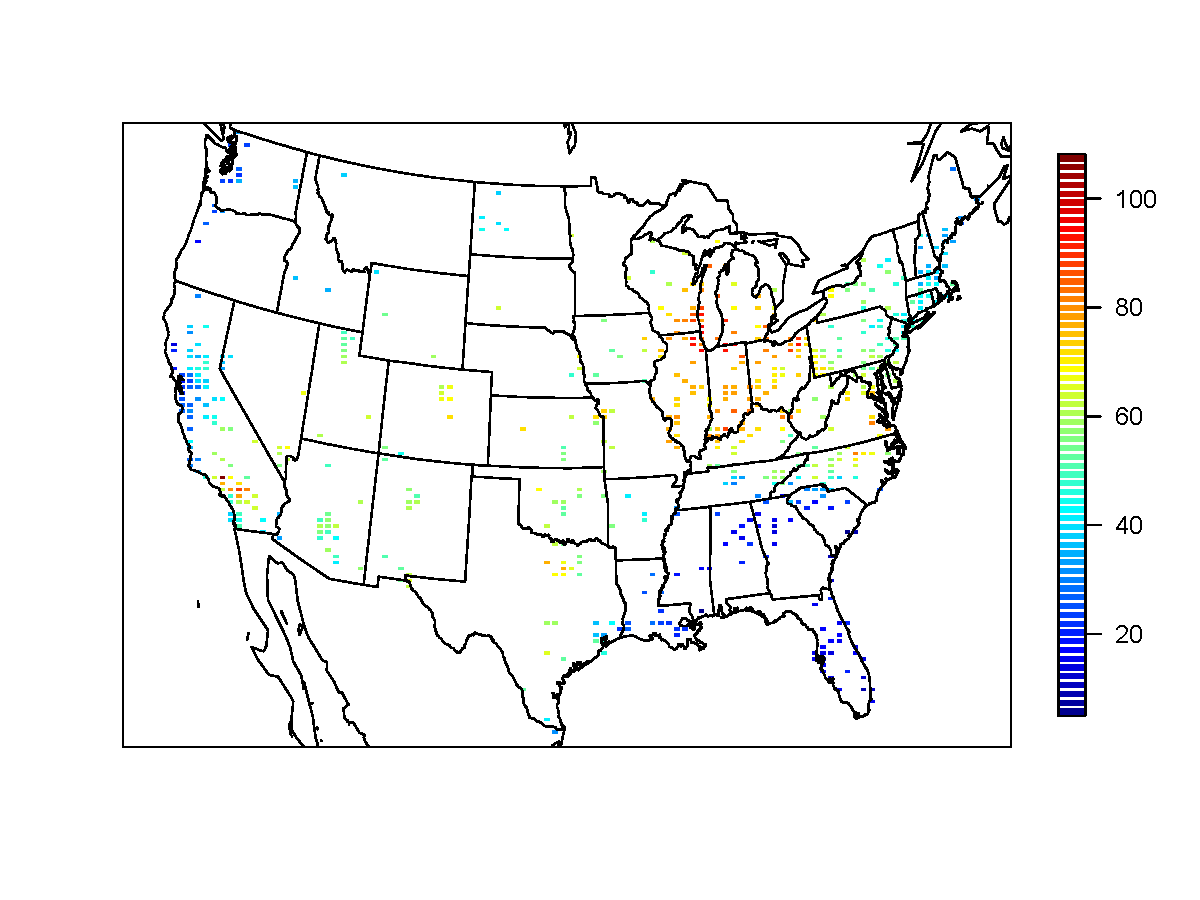
\includegraphics[width=0.75\linewidth]{plots/ozone-10jul-us.pdf}
  \caption{Ozone values (ppb) on July 10, 2005}
  \label{fig:ozone-10jul}
\end{figure}

A spatial model for threshold exceedances warrants special consideration and standard spatial methods are likely to perform poorly.
First, because we are interested only in high values, we want to ``let the tail speak for itself''.
That is, if we fit a model to the entire data set, low-to-moderate values would influence the fit of the overall model.
As there are more of these values, they can unduly influence the distribution at the higher levels about which we are interested.
Our inference method will only use data which exceed a threshold, and will impute data below the threshold, thereby tailoring the fit to the levels of interest.
Second, likelihood-based spatial modeling typically assumes a Gaussian process, which is appropriate when mean behavior is of interest.
However, the Gaussian distribution is light-tailed and symmetric, and therefore may be inappropriate for modeling data which does not share this tail behavior.
Third, we aim to capture the dependence structure when ozone is at high levels, and dependence at these levels may not be well-represented by covariances which focus again on mean behavior.
Asymptotic dependence/independence (see Section \ref{s:extdep}) are notions which describe how two random variables' probability of simultaneous exceedance of an extreme threshold behaves as one increases the threshold.
The Gaussian distribution always exhibits asymptotic independence, except in the case of perfect dependence, thus is an inappropriate model for data which exhibits asymptotic dependence.
To allow for more flexibility in the marginal tail and to allow for asymptotic dependence, the skew-$t$ distribution forms the basis for our model.

Our approach differs from threshold modeling approaches based on extreme value distributions.
There has been extensive work on threshold modeling in the field of extreme value statistics where extreme events are naturally defined in terms of exceedances over a high threshold.
\citet{Davison1990} considered modeling threshold exceedances of univariate time series by the generalized Pareto distribution.
Bivariate threshold models for extreme value distributions were considered by \citet{Ledford1996} who introduced a censored approach that provides a way to deal with different types of exceedances of a bivariate threshold in terms of only one or both components.
These threshold models were extended to spatial models for extremes by \citet{Wadsworth2012} and \citet{Thibaud2013} who fit various models to spatial extremes using a censored pairwise likelihood \citep{Padoan2010} based on the approach of \citet{Ledford1996}.
\citet{Huser2014} further extended this to space-time modeling.
\citet{Thibaud2013a}, \citet{Engelke2014}, and \citet{Wadsworth2014}, introduced more efficient inference for threshold exceedances of extremal spatial processes with full likelihood methods.
The previous approaches to threshold modeling are motivated by extreme value theory and assume the threshold is high enough that extremal models are valid for the data, and for extrapolation beyond the range of observed values.
Moreover, these approaches are computationally intensive and limited to rather small datasets.
For example, \citet{Wadsworth2014} present a simulation study with observations at 16 sites on a regular grid, and \citet{Engelke2014} analyze a dataset with observations at 35 meteorological stations.
Our application with ozone data does not fit into this framework because we do not focus on exceedances of a very high threshold, but on exceedances of a fixed threshold.
Furthermore, in our application, we have observations at over 1,000 ozone monitoring locations.

We propose a new spatiotemporal threshold exceedance model based on the skew-$t$ process \citep{Padoan2011}.
Our model is a threshold exceedance model for the multivariate skew-$t$ distribution for a fixed threshold.
In this setting, we describe the threshold as fixed because it is specified in advance by regulatory compliance.
This differs from the more traditional extremes literature where a threshold is selected to be the value beyond which an extremal model is appropriate for the data.
We use a skew-$t$ distribution because of its flexibility to model asymmetry and heavy-tailed data with the aim of predicting the probability of exceeding a high fixed threshold at an unobserved location.

Our model allows for inference and predictions using the full likelihood with computing on the order of Gaussian models for large space-time datasets.
This allows us to use Bayesian methods to impute data below the threshold as well as make predictions at unobserved locations.
In a spatial setting, the multivariate skew-$t$ distribution demonstrates asymptotic dependence between observations at all sites regardless of the distance between the sites.
In order to address this concern, we introduce a random spatial partition similar to the method used by \citet{Kim2005} for non-stationary Gaussian data.
This partitioning alleviates the asymptotic spatial dependence present in the skew-$t$ distribution for sites that are far apart.

The paper is organized as follows.
Section \ref{s:spatialskew} is a brief review of the spatial skew-$t$ process.
In Section \ref{s:spatial}, we build upon the traditional skew-$t$ process by incorporating censoring to focus on tails, partitioning to remove long-range asymptotic dependence, and extending the model to space-time data.
The computing is described in Section \ref{s:hier}.
In Section \ref{s:simstudy}, we present a simulation study that examines the predictive capabilities of this model compared Gaussian amd max-stable methods.
We then compare our method to Gaussian and max-stable methods with a data analysis of ozone measurements from 800 sites throughout the US in Section \ref{s:analysis}.
The final section provides brief discussion and direction for future research.

% These models describe dependence using the probability that two observations jointly exceed an extreme value, which in the limit of the distribution is referred to as asymptotic dependence.
% When the spatial domain is small, it may be reasonable to assume that all sites are asymptotically dependent; however for large spatial domains, it becomes more challenging to justify this assumption.
% This concern has been addressed by \citet{Wadsworth2012} in a spatial only setting and \citet{Huser2014} in a space-time setting.

% The main goal of our application is to estimate the marginal probability a site's ground-level ozone measurement will exceed 75 ppb.
% For July 2005, 75 ppb is approximately the 92nd sample quantile.
% However, if we look marginally at each site, 75 ppb is lower than the 90th quantile for almost 255 sites, and is below the median at 29 sites.
% The traditional threshold exceedance models arising from max-stable processes incorporate thresholding because the inference is only valid for very high values.
% Because 75 ppb represents such a wide range of marginal quantiles, these models based on max-stable methods may not be appropriate.

% Traditionally, spatial methods for extreme values analysis are conducted from one of two perspectives.
% The first of these is based on the convergence of the maximums of independent stochastic processes to a max-stable process \citep{deHaan2006}.
% Finite dimensional realizations of a max-stable process follow a generalized extreme value distribution \citep{Cooley2012}.
% One drawback to a block-maxima approach is that information is lost by discarding all but the most extreme observations in a block.
% Furthermore, in using multivariate block-maxima methods, the observations in the vector of block maxima rarely occur simultaneously \citep{Coles2001}.
% The other perspective incorporates a peaks-over-threshold approach.

% The use of multivarate models for threshold exceedances require evaluation of the underlying joint density.
% Finite dimensional realizations of max-stable processes are challenging to use because closed-form expressions for the density in more than two dimensions are complicated \citep{Coles1991}.
% One way to circumvent this challenge is to use pairwise composite likelihood methods \citep{Padoan2010}.
% When using pairwise composite likelihoods, threshold methods can then be implemented as long as the bivariate distribution can be evaluated \citep{Wadsworth2012,Thibaud2013,Huser2014}.
% Hierarchical models using Bayesian methods have also been proposed.
% For example, \citet{Reich2012} present a Bayesian hierarchical model, when conditioned on positive stable spatial random effects, the observations are independent.

% In certain settings, the multidimensional distributions are available.
% For example, \citet{Wadsworth2014} discuss a censored Poisson process that exploits the fact that the spectral functions for Brown-Resnick processes are log-Gaussian random fields.
% Additionally, \citep{Engelke2014}, show that upon standardizing marginals to the Gumbel distribution and conditioned on a fixed location exceeding a high threshold, the incremental distribution asymptotically forms a Gaussian process.
% In addition to Brown-Resnick processes, skew elliptical distributions can be used for multivariate modeling with dependent extreme values \citep{Genton2004,Zhang2010,Padoan2011}.
% For example, the skew-normal and skew-$t$ distribution offer a flexible way to handle non-symmetric data within a framework of multivariate normal and multivariate $t$ distributions.
% As with multivariate Gaussian distributions, the multivariate skew-normal distribution demonstrates asymptotic independence. Conversely both the multivariate $t$ and skew-$t$ distributions demonstrate asymptotic dependence \citep{Padoan2011}.
% Additionally, the limiting distribution of the maxima of skew-$t$ random vectors is the extremal skew-$t$ distribution \citep{Padoan2011} of which the extremal-$t$ \citep{Opitz2013} is a special case.

% Despite this challenge, spatial modeling is important because it provides a mechanism by which we can borrow information about extreme events across space.
% There are two primary goals for spatial methods.
% The first of these goals is to understand the marginal behavior at sites, and the second is to describe the dependence in the data.
% In many cases, these are done separately; however, with the development of pairwise composite likelihoods and Bayesian methods, it is resonable to model both simultaneously.
% One challenge to estimating the dependence in the tails of the distribution is that the dependence that present in the data may not be the same as the dependence in the limit of the underlying distribution \citep{Davison2012b}.
% Furthermore, in a spatial setting, it may be desirable to allow for varying degrees of tail dependence based upon the distance between two sites \citep{Wadsworth2012}.

\section{Spatial skew processes}\label{s:spatialskew}
The skew-elliptical family of distributions provides models that are mathematically tractable while introducing a slant parameter to account for asymmetric data \citep{Azzalini2014}.
A brief review of the additive process by which a skew-$t$ process is created is given here.

\subsection{Skew-$t$ process} \label{s:skewt}
Let $Y(\bs)$ be the observation at spatial location $\bs$ in a spatial domain of interest $\calD \in \calR^2$.
The spatial skew-$t$ process can be written
\begin{align}
  Y(\bs) = \bX(\bs)^T \bbeta + \lambda \sigma |z| + \sigma v(\bs)
\end{align}
where $\bX(\bs)$ is a set of spatial covariates at site $\bs$, $\bbeta$ is the vector of regression parameters, $\lambda \in \calR$ is a parameter controlling skew, $z \sim N(0, 1)$, $\sigma^2 \sim \text{IG}(a, b)$ is random scale parameter, IG is the distribution function of an inverse gamma random variable, and $v(\bs)$ is a spatial Gaussian process with mean zero, variance one, and a positive definite correlation function.

For a finite collection of locations $\bs_1, \ldots, \bs_n$, denote the vector of observations $\bY = [Y(\bs_1), \ldots, Y(\bs_n)]^T$.
After marginalizing over both $z$ and $\sigma$,
\begin{align}
  \bY \sim \text{ST}_n(\bX \bbeta, \bOmega, \balpha, 2a), \label{eq:fullmodel}
\end{align}
that is, $\bY$ follows an $n$-dimensional skew-$t$ distribution with location $\bX \bbeta$, correlation matrix $\bOmega$, slant parameters $\balpha$ and degrees of freedom $2a$, where $\bX = [\bX(\bs_1)^T, \ldots, \bX(\bs_n)^T]$, $\bOmega = \bomega \bar{\bOmega} \bomega$, $\bomega = \text{diag}\left(\frac{1}{ \sqrt{ab}}, \ldots, \frac{1}{\sqrt{ab}}\right)$, $\bar{\bOmega} = (\bSigma + \lambda^2 \bOne \bOne^T$), $\balpha = \lambda (1 + \lambda^2 \bOne^T \bSigma^{-1} \bOne)^{-1/2} \bOne^T \bSigma^{-1}$, and $\bSigma$ is the positive definite correlation matrix of $[v(\bs_1), \ldots, v(\bs_n)]$.
This process is desirable because of its flexible tail that is controlled by the skewness parameter $\lambda$ and degrees of freedom $2a$.
Furthermore, the marginal distributions at each location also follow a univariate skew-$t$ distribution \citep{Azzalini2014}.

Although any positive definite correlation function could be used, we choose to use the stationary isotropic \Matern correlation with
\begin{align}
  \text{cor}[v(\bs_1), v(\bs_2)] = \gamma I(\bs_1 = \bs_2) + (1 - \gamma)  \frac{ 1 }{ \Gamma(\nu) 2^{ \nu - 1}} \left( \sqrt{2\nu} \frac{ h }{ \rho } \right)^{\nu} K_{\nu} \left( \sqrt{2\nu} \frac{ h }{ \rho } \right) \label{eq:matern}
\end{align}
where $\rho$ is the spatial range, $\nu$ is the smoothness, $\gamma$ is the proportion of variance accounted for by the spatial variation, $K_\nu$ is a modified Bessel function of the second kind, and $h = || \bs_1 - \bs_2 ||$.
We use this parameterization for spatial correlation because the $\gamma$ parameter permits the inclusion of a nugget effect to account for non-spatial variability due to issues like measurement error.

\subsection{Extremal dependence}\label{s:extdep}
Our interest lies in spatial dependence in the tail of the skew-$t$ process.
One measure of extremal dependence is the $\chi$ statistic \citep{Coles1999}.
For a stationary and isotropic spatial process, the $\chi$ statistic for locations $\bs$ and $\bt$ separated by distance $h = || \bs - \bt ||$ with identical marginal distributions is
\begin{align}
  \chi(h) = \lim_{c \rightarrow c^*} \Pr[Y(\bs) > c | Y(\bt) > c]
\end{align}
where $c^*$ is the upper limit of the support of $Y$.
If $\chi(h) = 0$, then observations are asymptotically independent at distance $h$.
For Gaussian processes, $\chi(h) = 0$ regardless of the distance $h$, so they are not suitable for modeling asymptotically dependent extremes.
Unlike the Gaussian process, the skew-$t$ process is asymptotically dependent (the explicit expression for $\chi(h)$ is given in \ref{a:skewt}).
However, one problem with the spatial skew-$t$ process is that $\lim_{h \rightarrow \infty} \chi(h) > 0$.
This occurs because all observations, both near and far, share the same $z$ and $\sigma$ terms.
Therefore, this long-range dependence feature of the skew-$t$ process is not ideal for spatial analysis of large geographic regions where we expect only local spatial dependence.
We propose a solution to this in Section \ref{s:part}.

\section{Spatiotemporal skew-$t$ model for threshold exceedances}\label{s:spatial}
In this section, we propose extensions to the skew-$t$ process to model spatial extremes over a large geographic region by introducing censoring to focus on tail behavior and a random partition to remove long-range asymptotic dependence.
For notational convenience, we introduce the model for a single replication, and then extend this model to the spatiotemporal setting in Section \ref{s:temporal}.

\subsection{Censoring to focus on the tails}
As mentioned previously, we propose to use a censored approach because we are interested in high values and do not want the low-to-moderate values to influence the fit of the overall model.
% The censored observations below the threshold give information on the marginal probabilities to exceed the threshold and on the dependence, but their values are not used to fit the model.
Let
\beq\label{Yt}
  \widetilde{Y}(\bs) = \left\{ \begin{array}{ll}
      Y(\bs) \quad & \delta(\bs) = 1 \\
      T & \delta(\bs) = 0
  \end{array} \right.
\eeq
be the censored observation at site $\bs$ where $Y(\bs)$ is the uncensored observation, $\delta(\bs) = I[Y(\bs) > T]$, and $T$ is a pre-specified threshold value.
We impute the censored values as a step in the MCMC algorithm used to fit the model described in Section \ref{s:comp}.

\subsection{Partitioning to remove long-range asymptotic dependence}\label{s:part}
The motivation for the partition is that for a large spatial domain, it may not be reasonable to assume sites that are far apart demonstrate asymptotic dependence.
Modeling different levels of asymptotic dependence was discussed by \citet{Wadsworth2012} with a hybrid spatial dependence model.
\citet{Huser2014} also allow for varying asymptotic dependence across both space and time with a partition structure represented by random discs moving across the space for a random duration with a random velocity and random radius.
We handle the problem of long-range asymptotic dependence with a random partition.
As discussed in Section \ref{s:spatialskew}, the source of long-range dependence is the shared $z$ and $\sigma$.
Therefore, to alleviate this dependence, we allow $z$ and $\sigma$ to vary by site.
The model becomes
\begin{align} \label{eq:partition}
  Y(\bs) &= \bX(\bs)^T \bbeta + \lambda \sigma(\bs) |z(\bs)| + \sigma(\bs) v(\bs).
\end{align}
To model spatial variation, consider a set of spatial knots $\bw_1, \ldots, \bw_K$ from a homogeneous Poisson process with intensity $\mu$ over spatial domain $\calD \in \calR^2$.
The knots define a random partition of $\calD$ by subregions $P_{1}, \ldots, P_{K}$ defined as
\begin{align} \label{eq:subregions}
  P_{k} = \{ \bs : k = \argmin_\ell || \bs - \bw_{\ell} || \}.
\end{align}
All $z(\bs)$ and $\sigma(\bs)$ for sites in subregion $k$ are assigned common values
\begin{align}
  z(\bs) = z_{k} \quad \text{and} \quad \sigma(\bs) = \sigma_{k} \label{eq:sitezsig}
\end{align}
and the $z_k$ and $\sigma^2_k$ are distributed as $z_k \iid N(0, 1)$ and $\sigma^2_k \iid$ IG$(a, b)$.
So, within each partition, $Y(\bs)$ follows the spatial skew-$t$ process defined in Section \ref{s:spatialskew}.
Across partitions, the $Y(\bs)$ remain correlated via the correlation function for $v(\bs)$ because $v(\bs)$ spans all partitions.

The partitioning model remove long-range dependence. Conditional on knots $\bw_1, \ldots, \bw_K$, the $\chi$ statistic for two sites $\bs$ and $\bt$ in partitions $k_s$ and $k_t$ respectively is
\begin{align}
  \chi(h) &= I(k_s = k_t) \chi_{\text{skew-}t}(h) + I(k_s \neq k_t) \chi_{\text{Gaus}}(h) \nonumber \\
         &= I(k_s = k_t) \chi_{\text{skew-}t}(h)
\end{align}
where $I(\cdot)$ is an indicator function, $\chi_{\text{skew-}t}(h)$ is the $\chi$ statistic for a skew-$t$ process given in (\ref{eq:chiskew-t}), $\chi_{\text{Gaus}}(h)$ is the $\chi$ statistic for a Gaussian process, and $h = ||\bs - \bt||$.
Therefore, sites in different subregions are asymptotically independent because $\chi_{\text{Gaus}}(h) = 0$ for all $h$.
Marginally, over the knots, $\chi(h) = \pi(h) \chi_{\text{skew}-t}(h)$, where $\pi(h) = \Pr(k_s = k_t)$ is the probability that two sites separated by distance $h$ are in the same partition.
In \ref{a:proofsamepartition}, we show that $\lim_{h \rightarrow \infty} \pi(h) = 0$, implying $\lim_{h \rightarrow \infty} \chi(h) = 0$.
In Figure \ref{fig:chi}, we give $\chi(h)$ for $K = 1, 3, 5, 10$ partitions for a skew-$t$ distribution with $\alpha = 10$, and 3 degrees of freedom.
In Figure \ref{fig:chi} we estimate $\pi(h)$ through simulation.
% To estimate $\pi(h)$, we generate 500 sites uniformly over the unit-square.
% We then randomly generate 400 different sets of partitions using $K = 3$, $5$, and $10$.
% For each set of knots, we take $\pi(h)$ to be the proportion of sites in the same partition that are separated by distance $h$.
% This plot demonstrates how partitioning helps to reduce extremal dependence as $h$ increases.

\begin{figure}
  \centering
  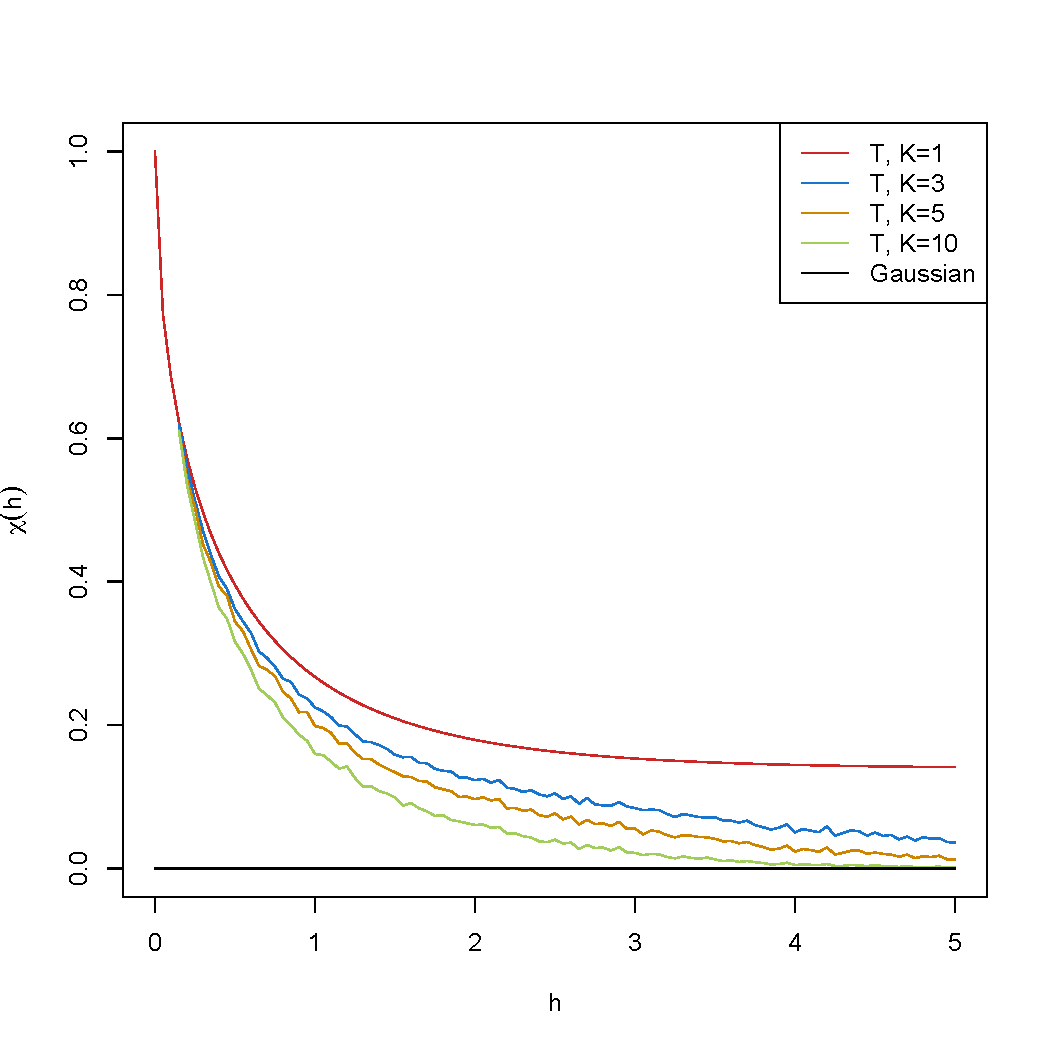
\includegraphics[width=0.5\linewidth]{plots/chi-h.pdf}
  \caption{Extremal dependence measure $\chi(h)$, as a function of distance, $h$, for $K = 1, 3, 5$, and $10$ knots.}
  \label{fig:chi}
\end{figure}

\subsection{Extension to space-time data} \label{s:temporal}
When using daily measurements, the assumption of temporal independence is often inappropriate.
In this section, we extend (\ref{eq:partition}) to the spatiotemporal setting.
There are several places where temporal dependence could be incorporated in the model, including the residuals $v_t(\bs)$.
However, we choose to allow for temporal dependence in the $\bw$, $z$, and $\sigma$ terms because these terms dictate the tail behavior which is our primary focus.
Let
\begin{align} \label{eq:spatiotemp}
  Y_t(\bs) = \bX_t(\bs)^T \bbeta + \lambda \sigma_t(\bs) |z_t(\bs)| + \sigma_t(\bs) v_t(\bs),
\end{align}
where $t \in \{1, \ldots, T\}$ denotes the day of each observation.
Let \hbox{$\bw_{tk} = (w_{tk1}, w_{tk2})$} be a spatial knot on day $t$, and let $w_{t1}, \ldots, w_{tK}$ be a collection of spatial knots on day $t$.
As in Section \ref{s:part}, these knots define a daily partition $P_{t1}, \ldots, P_{tK}$, and for $\bs \in P_{tk}$,
\begin{align}
  z_t(\bs) = z_{tk}\quad \text{and} \quad \sigma_{t}(\bs) = \sigma_{tk}.
\end{align}
We allow the partition structure to vary from day to day in order to account for sharp spikes in a response that may not be present every day (e.g. the impact of a forest fire on ozone levels).

We use an AR(1) time series model for $w_{tk}$, $z_{tk}$, and $\sigma_{tk}$.
The time series model must be specified after a transformation to preserve the skew-$t$ process at each time point.
For each time-varying parameter, we transform to obtain a standard normal marginal distribution, place a Gaussian prior with autocorrelation on the transformed parameter, and then transform back to the appropriate marginal distribution for the skew-$t$ process.
We first transform the spatial knots from $\calD$ to $\calR^2$ as follows.
Let
\begin{align}
  w^*_{tki} = \Phi^{-1}\left[ \frac{ w_{tki} - \min(\bs_i)}{ \max(\bs_i) - \min(\bs_i) } \right], \quad i = 1, 2
\end{align}
where $\Phi$ is a univariate standard normal density function and $\bs_i = [s_{1i}, \ldots, s_{ni}]$.
Then the transformed knots $\bw^*_{tk} \in \calR^2$.
We use a copula on $\sigma^2_t(\bs)$ to ensure that the marginal distributions of $\sigma^2_t(\bs)$ are inverse gamma.
Let
\begin{align}
  \sigma^{2*}_t(\bs) =\Phi^{-1}\left\{ \text{IG}[\sigma^2_t(\bs)] \right\}
\end{align}
where IG is defined as before.
We also use a copula on $z_{t}(\bs)$ to ensure that the marginal distributions of $z_t(\bs)$ are half-normal.
Let
\begin{align}
  z^*_t(\bs) = \Phi^{-1}\left\{ \text{HN}[z_t(\bs)] \right\}
\end{align}
where HN is the distribution function of a half-normal random variable.
The AR(1) process for each tail parameter is $\bw^*_{1k} \sim N_w(0, 1)$, $z^*_{1k} \sim N(0, \sigma^2_{1k})$, $\sigma^{2*}_{1k} \sim N(0, 1)$, and for $t > 1$ the time series is modeled as
\begin{align}
  \bw^*_{tk} | \bw^*_{t-1, k} &\sim N_2\left[\phi_w \bw^*_{t-1, k}, (1 - \phi_w^2) \right] \\
  z^*_{tk} | z^*_{t-1, k} &\sim N \left[\phi_z z^*_{t-1, k}, \sigma^2_{tk} (1 - \phi_z^2)\right] \\
  \sigma^{2*}_{tk} | \sigma^{2*}_{t-1, k} &\sim N \left[\phi_\sigma \sigma^{2*}_{t-1, k}, (1 - \phi_\sigma^2) \right]
\end{align}
where $|\phi_w|$, $|\phi_z|$, $|\phi_\sigma| < 1$.
These are stationary time series models with marginal distributions \hbox{$\bw^*_{k} \sim N_2(0, 1)$}, \hbox{$z^*_{k} \sim N(0, \sigma^2_{k})$}, and \hbox{$\sigma^{2*}_{k} \sim N(0, 1)$}.
After transformation back to the original space, $\bw_{tk} \sim \text{Unif}(\calD)$, $z_{tk} \sim HN(0, \sigma^2_{tk})$ $\sigma^2_{tk} \sim \text{IG}(a, b)$.
For each day, the model is identical to the spatial-only model in (\ref{eq:partition}) by construction.

\section{Hierarchical model}\label{s:hier}
Conditioned on $z_{tk}(\bs)$, $\sigma^2_{tk}(\bs)$, and $P_{tk}$, the marginal distributions are Gaussian and the joint distribution multivariate Gaussian.
However, we do not fix the partitions, they are treated as unknown and updated in the MCMC algorithm.
We model this with a Bayesian hierarchical model as follows.
Let $\bw_{t1}, \ldots, \bw_{tK}$ be a set of daily spatial knots in a spatial domain of interest, $\calD$, and $P_{tk}$ as defined in (\ref{eq:subregions}).
In practice, we fix $K$ at different levels, and assess its impact on prediction as described in \ref{s:modelselect}.
Then
\begin{align}
   Y_t(\bs) \mid z_{t}(\bs), \sigma_t^2(\bs), P_{tk}, \Theta &= \bX_t(\bs)^T \beta + \lambda |z_t(\bs)| + \sigma_t(\bs) v_t(\bs) \label{eq:hier}\\
   z_t(\bs) &= z_{tk} \text{ if } \bs \in P_{tk}\nonumber\\
   \sigma^2_{t}(\bs) &= \sigma^2_{tk} \text{ if } \bs \in P_{tk}\nonumber\\
   \lambda &= \lambda_1 \lambda_2\nonumber\\
   \lambda_1 &= \left\{ \begin{array}{ll}
      +1 \quad & \text{w.p. } 0.5\\
      -1 \quad & \text{w.p. } 0.5
   \end{array}\right.\nonumber\\
   \lambda^2_2 & \sim IG(a, b)\nonumber\\
   v_t(\bs) \mid \Theta &\sim \Matern(0, \Sigma)\nonumber\\
   z^*_{tk} \mid z^*_{t-1, k}, \sigma^2_{tk} &\sim N(\phi_z z^*_{t-1, k}, \sigma^2_{tk} (1 - \phi_z^2))\nonumber\\
   \sigma^{2*}_{tk} \mid \sigma^{2*}_{t-1, k} &\sim N(\phi_\sigma \sigma^{2*}_{t-1, k}, (1 - \phi_\sigma^2))\nonumber\\
   \bw^*_{tk} \mid \bw^*_{t-1, k} &\sim N_2(\phi_w \bw^*_{t-1, k}, (1 - \phi_w^2)) \nonumber
\end{align}
where $\Theta = \{\rho, \nu, \gamma\, \lambda, \beta\}$, and $\Sigma$ is a \Matern covariance matrix as described in Section \ref{s:skewt}.
We parameterize $\lambda = \lambda_1 \lambda_2$ to help with convergence in the MCMC.

\subsection{Computation}\label{s:comp}
We use MCMC methods to explore the posterior.
At each MCMC iteration, we first impute values below the threshold conditional on observations above the threshold.
This is feasible for large datasets with our model because for a single day, conditional on the model parameters, we only need to draw from a truncated multivariate normal distribution.
We can use Gibbs sampling to update $Y_t(\bs)$ for censored observations that are below the threshold $T$.
After conditioning on $\lambda$, $z_t(\bs)$ and non-censored observations, $Y_t(\bs)$ has truncated normal full conditionals.
So we sample $Y_t(\bs) \sim N_{(-\infty, T)}(\bX_t^T(\bs) \beta + \lambda | z_t(\bs)|, \bSigma)$.

Then, we update model parameters, $\Theta$, using a Metropolis-Hastings algorithm with Gibbs sampling when needed.
The final step of the computation is to use Bayesian Kriging to generate a predictive distribution for $Y_t(\bs^*)$ at prediction location $\bs^*$.
This step is similar to the imputation for censored observations except that the full conditionals are no longer truncated at $T$.
See Appendices A.1 and A.2 for details regarding the MCMC algorithm.

\section{Simulation study}\label{s:simstudy}
In this section, we present the results from a simulation study to investigate how the number of partitions and the level of thresholding impact the accuracy of predictions made by the model and to compare with Gaussian and max-stable methods.

\subsection{Design}\label{s:simdesign}
For all simulation designs, we generated data from model (\ref{eq:partition}) in Section \ref{s:part} using $n_s=144$ sites and $n_t=50$ independent days.
The sites were generated Uniform$([0, 10] \times [0, 10])$.
We generated data from 4 different simulation designs:
\begin{enumerate} \setlength{\itemsep}{-0.5em}
  \item Gaussian marginal, $K=1$ knot
  % \item Symmetric-$t$ marginal, $K=1$ knot
  % \item Symmetric-$t$ marginal, $K=5$ knots
  \item Skew-$t$ marginal, $K=1$ knots
  \item Skew-$t$ marginal, $K=5$ knots
  \item Max-stable
  % \item Transformation below $T = q(0.80)$
\end{enumerate}
In the first three designs, the $v_t(\bs)$ terms were generated using a \Matern covariance with smoothness parameter $\nu = 0.5$ and spatial range $\rho = 1$.
For the covariance matrices in designs 1 -- 3, the proportion of the variance accounted for by the spatial variation was $\gamma = 0.9$ while the proportion of the variance accounted for by the nugget effect was $0.1$.
In the first design, $\sigma^2 = 2$ was used for all days which results in a Gaussian distribution.
For designs 2 and 3, $\sigma^2_{tk} \iid \text{IG}(3, 8)$ to give a $t$ distribution with 6 degrees of freedom.
For design 1, we set $\lambda = 0$.
For designs 2 and 3, $\lambda = 3$ was used as to simulate moderate skewness, and the $z_t$ were generated as described in (\ref{eq:sitezsig}).
In designs 1 -- 3, the mean $\bX^T \bbeta = 10$ was assumed to be constant across space.
In the fourth design, we generated from a spatial max-stable distribution \citep{Reich2012}.
In this design, data have marginal distributions that follow a generalized extreme value distribution with location parameter $1$, scale parameter $1$, and shape parameter $0.2$.
In this model, a random effect was used to induce spatial dependence using 144 spatial knots on a regular lattice in the square $[1, 9] \times [1, 9]$.
For this setting, $\gamma_{\text{RS}} \in (0, 1)$, is similar to $\gamma$ in that it controls the relative strength of the nugget effect.
We set $\gamma_{\text{RS}} = 0.5$, which represents moderate spatial dependence.
% In the final design, we generate $\tilde{y}$ using the setting from design 2, and then transform the data
% \begin{align}
%   y = \left\{ \begin{array}{lc}
%     \tilde{y}, \quad & \tilde{y} > T \\[0.5em]
%     T \exp\{\tilde{y} - T\}, \quad & \tilde{y} \le T
%   \end{array}\right.
% \end{align}
% where $T = q(0.80)$ is the 80th sample quantile of the data.
% The final design is included to explore the importance of using a threshold exceedance model when the distribution for the bulk of the data is misspecified.


$M = 50$ data sets are generated for each design.
For each data set we fit the data using six models
\begin{enumerate} \setlength{\itemsep}{-0.5em}
  \item Gaussian marginal, $K=1$ knots
  \item Skew-$t$ marginal, $K=1$ knots, $T=-\infty$
  \item Symmetric-$t$ marginal, $K=1$ knots, $T=q(0.80)$
  \item Skew-$t$ marginal, $K=5$ knots, $T=-\infty$
  \item Symmetric-$t$ marginal, $K=5$ knots, $T=q(0.80)$
  \item A max-stable model based on \citet{Reich2012} thresholded at $T = q(0.80)$
\end{enumerate}
where $q(0.80)$ is the 80th sample quantile of the data.
The design matrix $\bX$ includes an intercept with a first-order spatial trend with priors of $\beta_\text{int}$, $\beta_\text{lat}$, $\beta_\text{long},  \iid \text{N}(0, 10)$.
The spatial covariance parameters have priors $\log(\nu) \sim \text{N}(-1.2, 1)$, $\gamma \sim \text{Unif}(0, 1)$, $\rho \sim \text{Unif}(15)$.
The skewness parameter has prior $\lambda_2 \sim \text{IG}(0.1, 0.1)$.
The residual variance terms have priors $\sigma^2_t(\bs) \sim \text{IG}(a, b)$, where $a$ has a Gamma$(0.1, 0.1)$ prior and $b$ has a discrete uniform prior on a mesh from $0.1$ to $10$ with spacing of $0.1$.
The knots have priors $\bw \sim \text{Unif}(\calD)$.
We tried also fitting the skew-$t$ marginals for the thresholded models, but it is very challenging for the MCMC to properly identify the skewness parameter with a censored left tail.
Each chain of the MCMC ran for 20,000 iterations with a burn-in period of 10,000 iterations.
Parameters appear to converge properly; however, in the models with multiple partitions (i.e. models 4 and 5) it is hard to assess the convergence of $\bw$, $z(\bs)$, and $\sigma^2(\bs)$ because of partition label switching throughout the MCMC.

\subsection{Cross validation}\label{s:modelselect}
Models were compared using cross validation, with 100 sites used as training sites to fit the models, and 44 sites withheld for testing the predictions.
Because one of the primary goals of this model is to predict exceedances over a fixed threshold, we use Brier scores to compare the models \citep{Gneiting2007}.
The Brier score for predicting exceedance of a threshold $c$ is given by $[e(c) - P(c)]^2$ where $e(c) = I[y>c]$ is an indicator function indicating that a test set value, $y$, has exceeded the threshold, $c$, and $P(c)$ is the predicted probability of exceeding $c$.
We average the Brier scores over all test sites and days.
For the Brier score, a lower score indicates a better fit.

\subsection{Results}\label{s:simresults}
We compared the Brier scores for exceeding 4 different thresholds for each dataset.
The thresholds used for the Brier scores are extreme quantiles from the simulated data for $q(0.90)$, $q(0.95)$, $q(0.98)$, and $q(0.99)$.
Figure \ref{fig:simbrierscores} gives the Brier score relative to the Brier score for the Gaussian method calculated as
\begin{align}
  \text{BS}_{\text{rel}} = \frac{\text{BS}_{\text{method}}}{\text{BS}_{\text{Gaussian}}}.
\end{align}
We analyzed the results for the simulation study using a Friedman test at $\alpha = 0.05$ to see if at least one method had a significantly different Brier score.
For Friedman tests that came back with a significant p-value, we conducted a Wilcoxon-Nemenyi-McDonald-Thompson test to see which of the methods had different results.
The full results for the Wilcoxon-Nemenyi-McDonald-Thompson tests are given in \ref{a:pdiffs}.

The results show that when the data are generated from a Gaussian process, our method performs comparably to a Gaussian approach.
In general, when the underlying process is not Gaussian, our method results in an improvement over both the max-stable and Gaussian methods.
One exception to this is the case when the generative process is max-stable.
In this case, the max-stable method outperforms our method; however, for predictions at high quantile levels, the differences between the max-stable method and our method decrease.
The non-thresholded methods tend to outperform the thresholded methods, but this is not surprising given that in most cases, the data are generated directly from the model used in the method.
% Finally, for setting 5, although the thresholded version of the single-partition model tends to perform the best across all of the extreme quantiles, the difference between the thresholded and non-thresholded methods is no longer significant in the more extreme quantiles.
In summary, our method provides more flexibility for data that demonstrate some level of asymmetry or heavy tails, while still performing comparably to Gaussian methods when the data are symmetric and have light tails.

\begin{figure}
  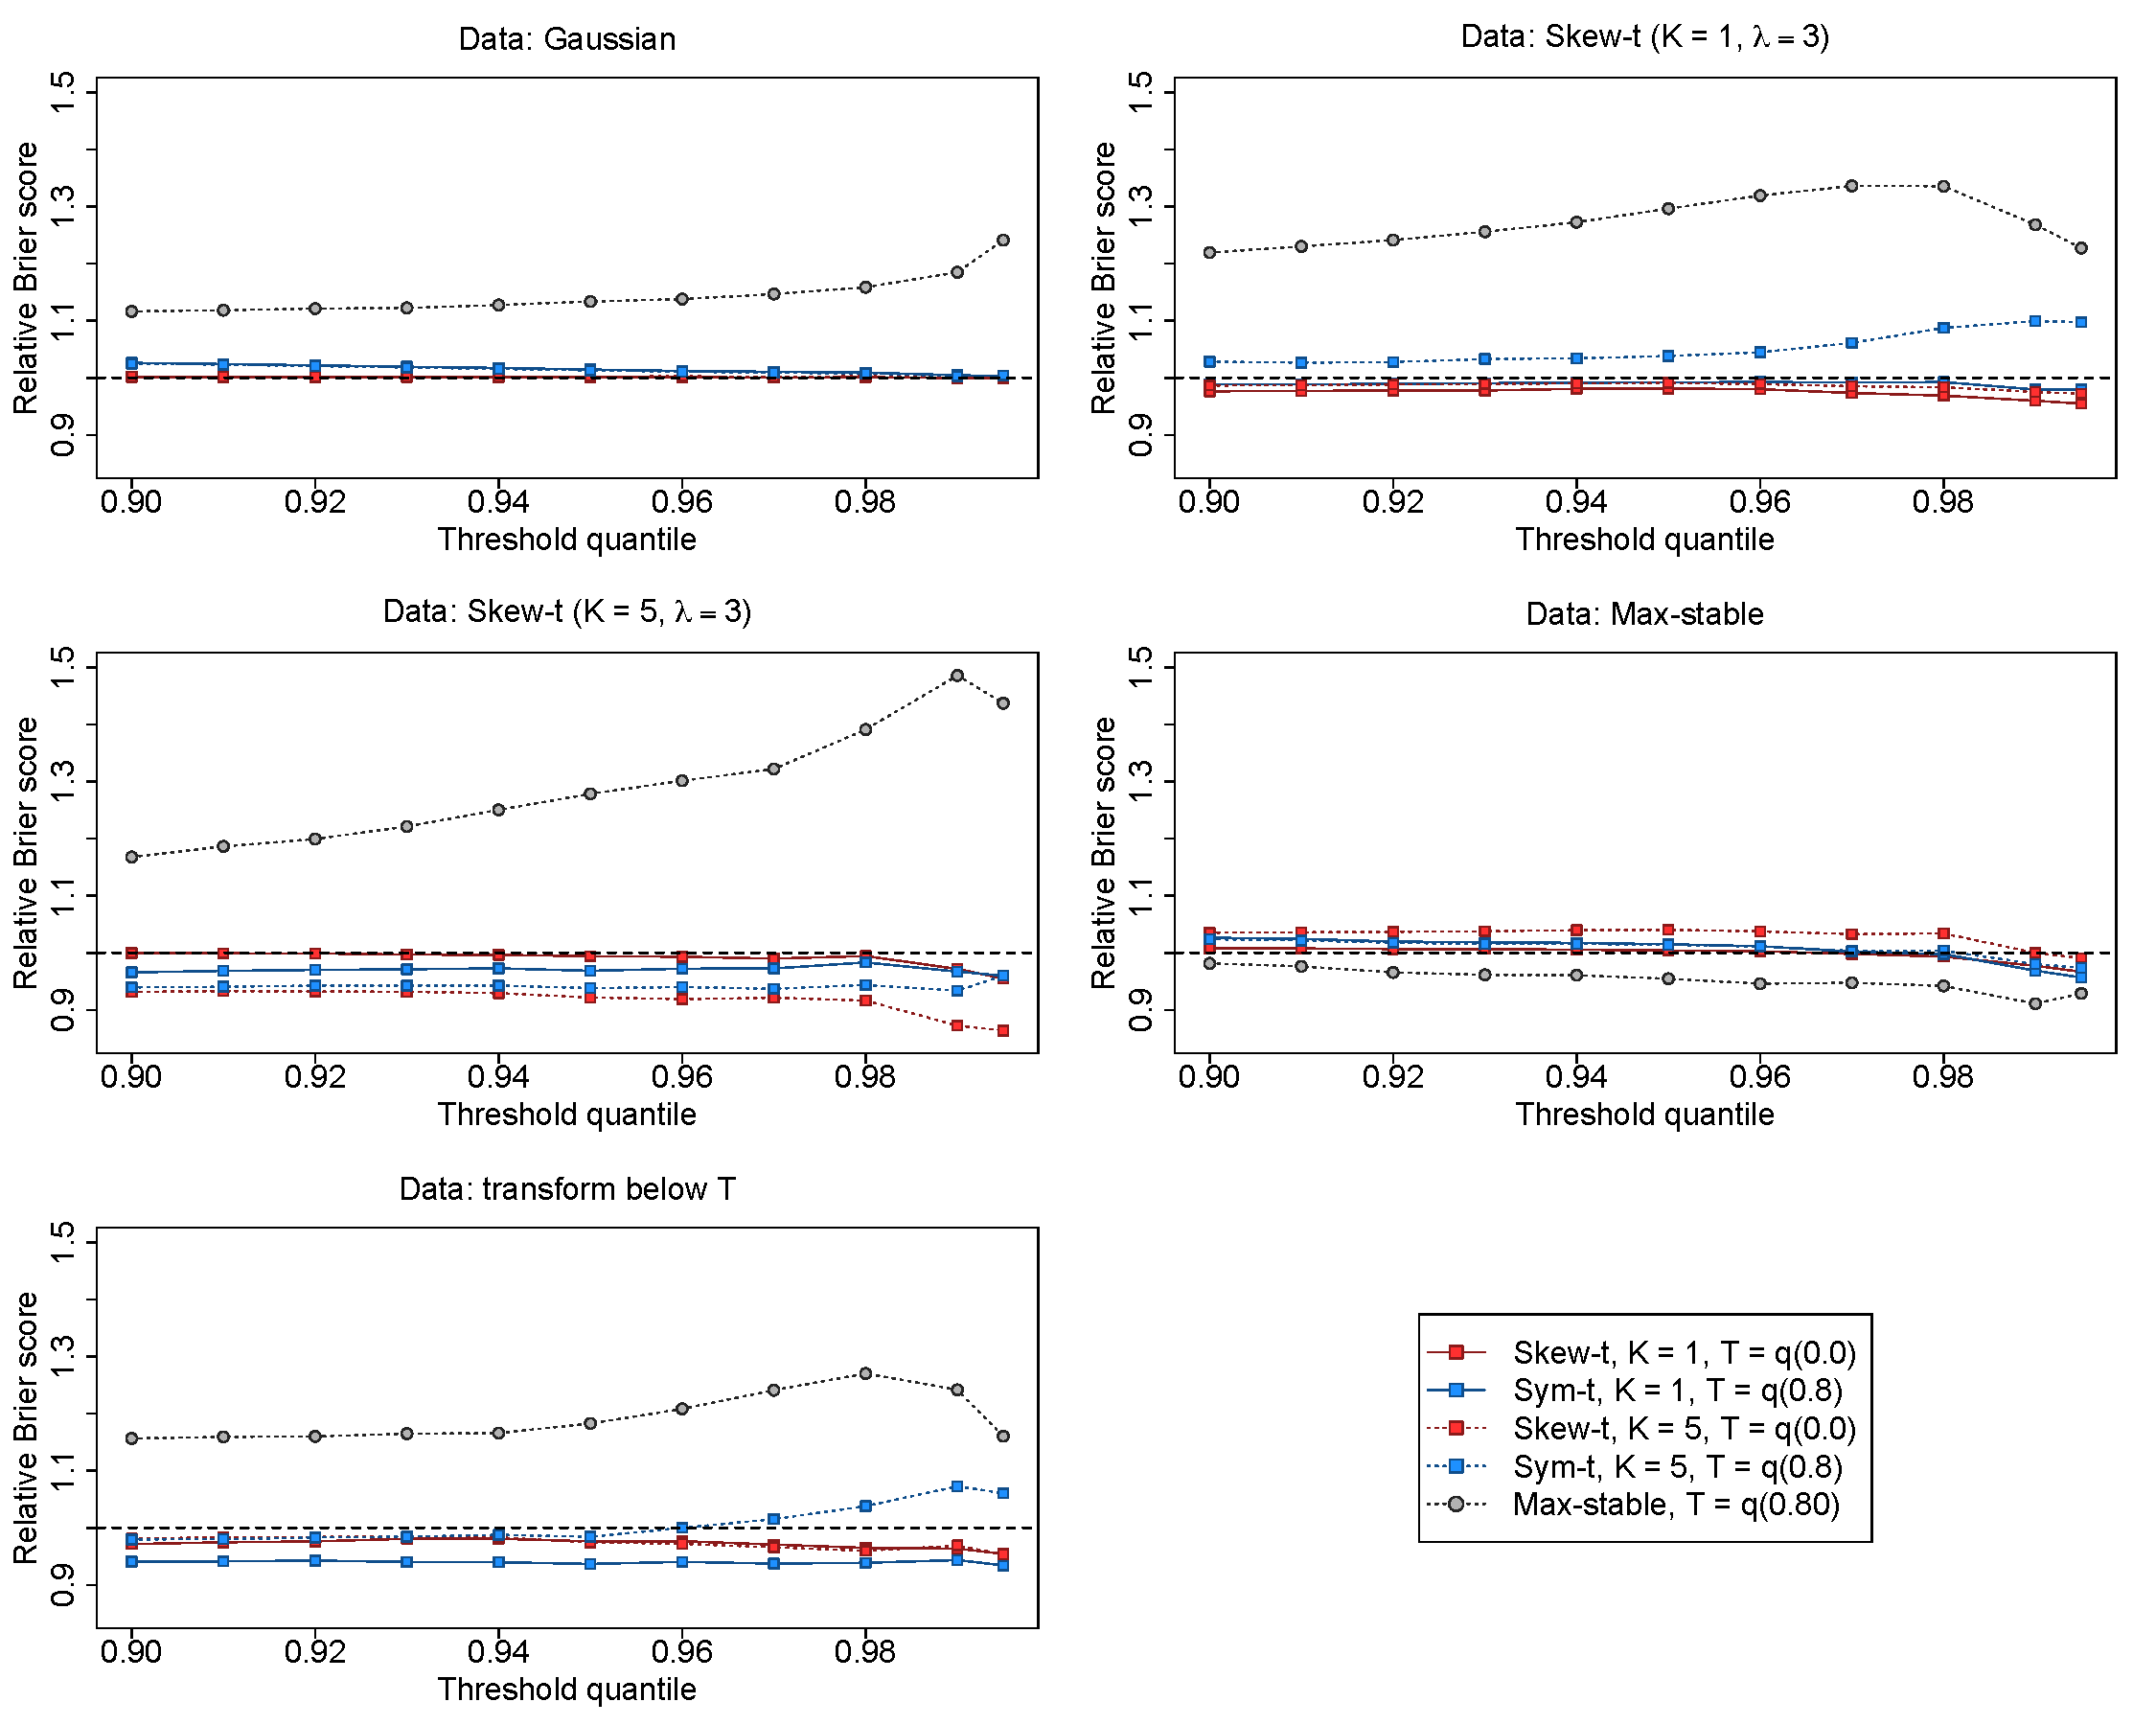
\includegraphics[width=\linewidth]{plots/bsplots-mean.pdf}
  \caption{Brier scores relative to the Gaussian method for simulation study results. A ratio lower than 1 indicates that the method outperforms the Gaussian method.}
  \label{fig:simbrierscores}
\end{figure}

\section{Data analysis}\label{s:analysis}
We consider daily observations of maximum 8-hour ozone measurements for the 31 days of July 2005 at 1,089 Air Quality System (AQS) monitoring sites in the United States as the response (see Figure \ref{fig:ozone-10jul}).
For each site, we also have covariate information containing the estimated ozone from the Community Multi-scale Air Quality (CMAQ) modeling system.
Initially, we fit a linear regression assuming a mean function of
\begin{align}
  \text{E}[Y_i(\bs)] = \beta_0 + \beta_1 \cdot \text{CMAQ}_t(\bs). \label{eq:datamean}
\end{align}
Figure \ref{fig:ozone-qq} shows a Q-Q plot of the residuals compared to a skew-$t$ distribution with 10 d.f. and $\alpha = 1$.
\begin{figure}
  \centering
  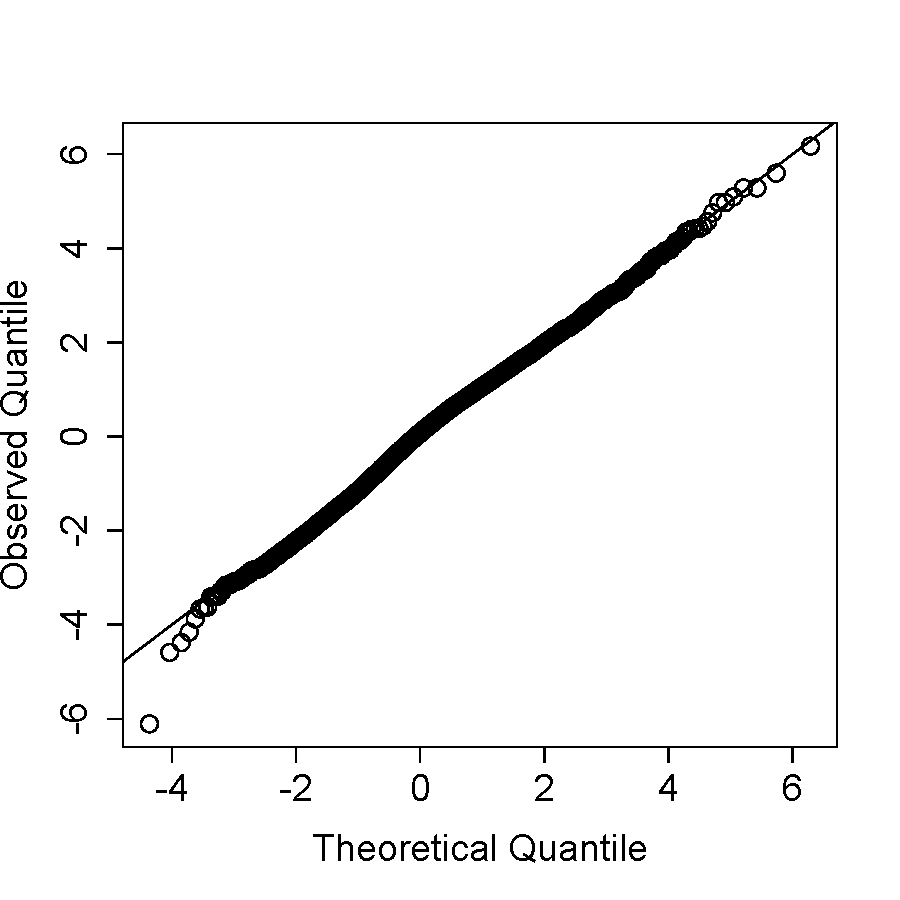
\includegraphics[width=0.5\linewidth]{plots/qq-res.pdf}
  \caption{Q-Q plot of the residuals for a skew-$t$ distribution with 10 d.f. and $\alpha = 1$ (right)}
  \label{fig:ozone-qq}
\end{figure}

Standard exploratory data analysis techniques for extremal dependence are very challenging with only 31 days worth of data because it is difficult to estimate extreme quantiles at each site to obtain empirical estimates of $\chi$.
Despite the fact that there is only one month of data, we can get some sense of extremal dependence between sites by looking at joint occurrences of high sample quantiles.
For example, Figure \ref{fig:bivariateozone} suggests there is more agreement between sites that are close to one another than sites that are far from one another.
\begin{figure}
  \centering
  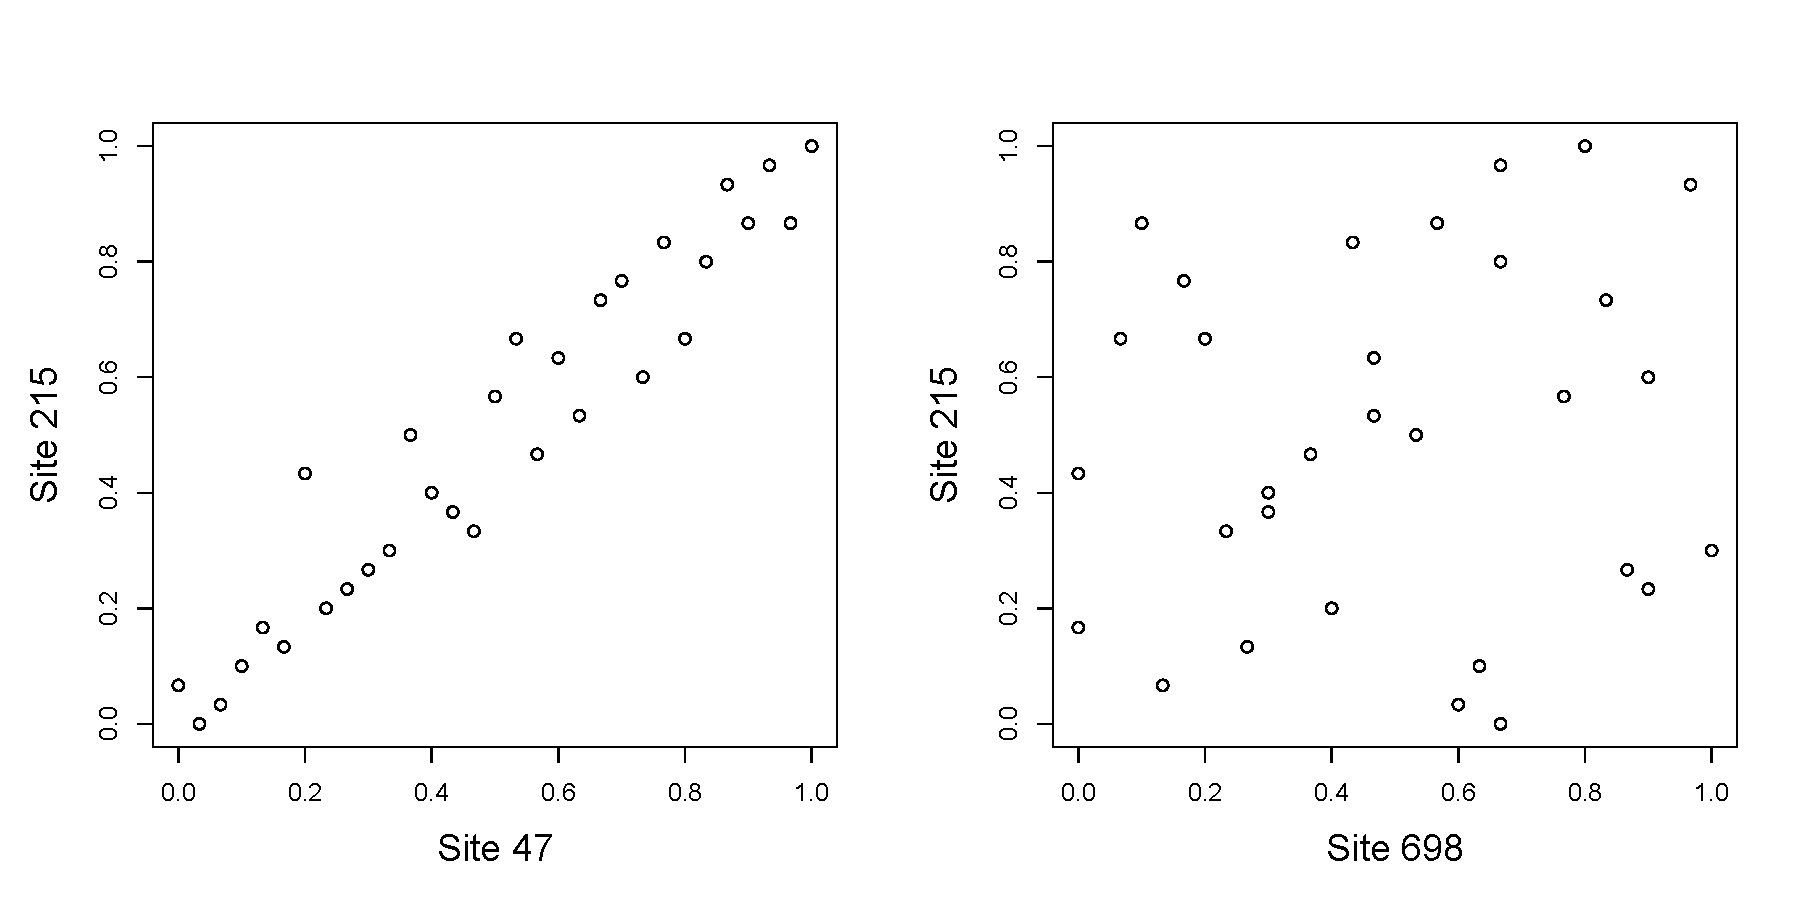
\includegraphics[width=\linewidth]{plots/daily-quantiles-ozone.pdf}
  \caption{Daily quantiles for two monitoring locations near Columbus, OH (left) and daily quantiles for a monitoring location in Los Angeles, CA and Columbus, OH (right)}
  \label{fig:bivariateozone}
\end{figure}
Another aspect that distinguishes our approach from more traditional extremes analyses, is how the threshold is selected.
In our example, a threshold of 75 ppb which corresponds to $q(92)$ for all observations, but marginally it represents anywhere from $q(0.06)$ to $q(1)$.

% We explore spatial and temporal extremal dependence by considering $\chi_c = \Pr[Y(\bs) > c | Y(\bt) > c]$.
% To examine spatial dependence in high quantiles, we consider observations at all pairs of sites $\bs$ and $\bt$ that are distance $h$ apart where $h$ is separated into bins of size 0.25 km.
% Then conditioned on $Y(\bt) > c$, we take the sample proportion of $Y(\bs) > c$.
% Finally, $\widehat{\chi}_c(h)$ is averaged over all days at each of the three threshold quantiles.
% To examine temporal dependence in high quantiles, we consider observations at a single site that are taken lag-$t$ days apart.
% Then conditioned on $Y_n(\bs) > c$, we take the sample proportion of $Y_{n + t}(\bs) > c$.
% Finally, $\widehat{\chi}(t)$ is averaged over all sites at each of the three threshold quantiles.
% The $\widehat{\chi}_c(h)$ and $\widehat{\chi}_c(t)$ plots in Figure \ref{fig:chi-st} show the estimated spatial and temporal dependence of the residuals for the ozone data at three quantile levels $q(0.90), q(0.95)$, and $q(0.99)$.

% \begin{figure}
%   \centering
%   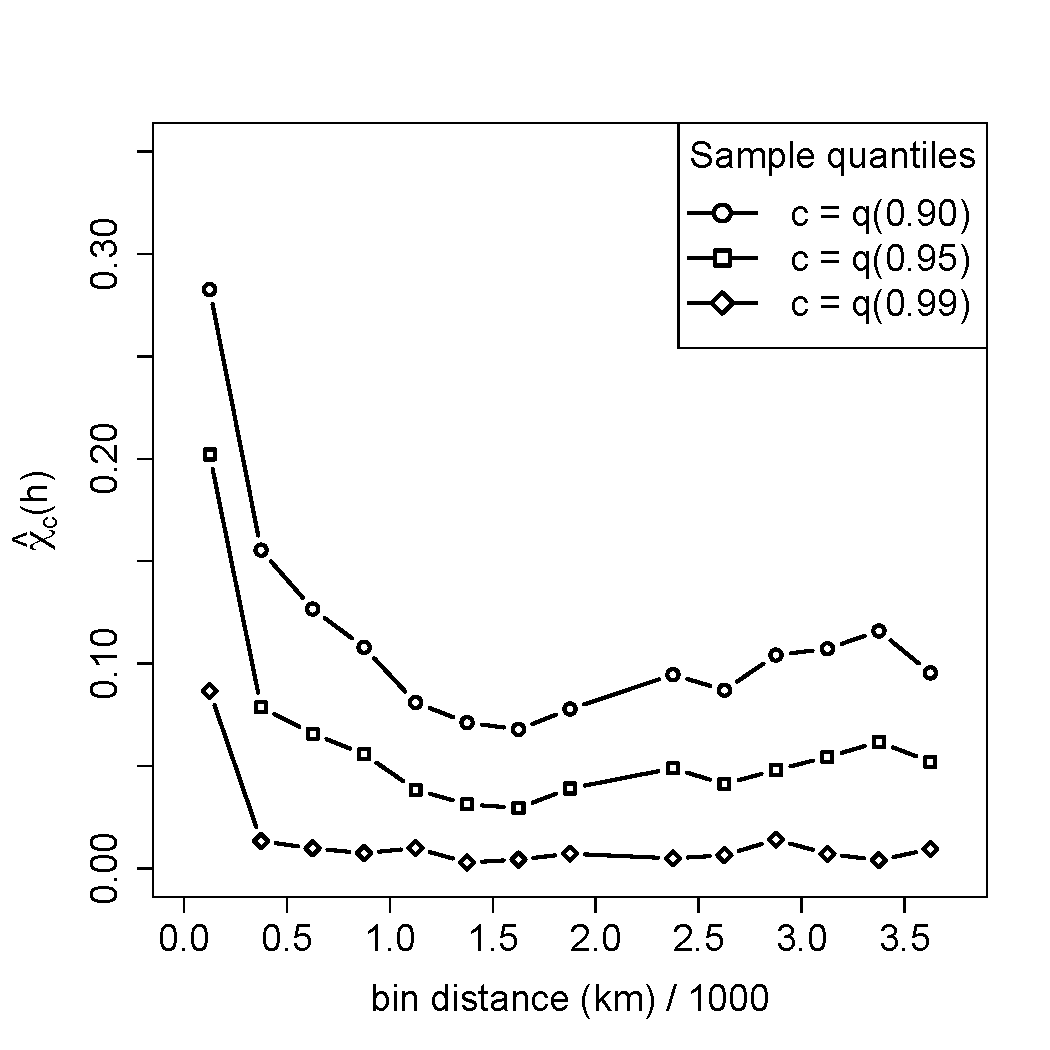
\includegraphics[width=0.49\linewidth]{plots/chi-h-ozone.pdf}
%   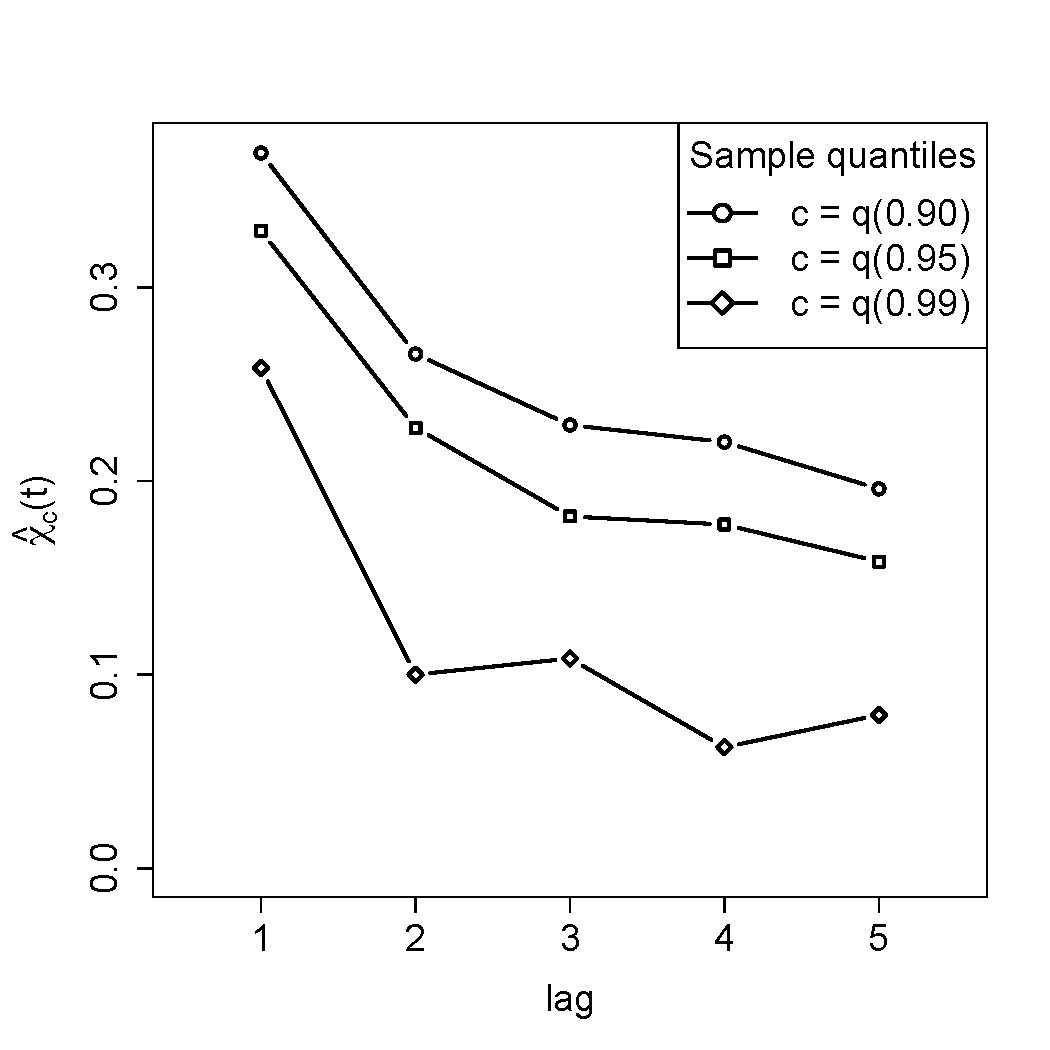
\includegraphics[width=0.49\linewidth]{plots/chi-t-ozone.pdf}
%   \caption{$\widehat{\chi}_c(h)$ plot for the residuals (left). $\widehat{\chi}_c(t)$ plot for the residuals (right).}
%   \label{fig:chi-st}
% \end{figure}

\subsection{Model comparisons}
We fit the model using Gaussian and skew-$t$ marginal distributions with $K=1, 5, 6, 7, 8, 9, 10, 15$ partitions.
We choose to censor $Y(\bs)$ at $T = 0$, $T = 50$ (0.42 sample quantile), and $T = 75$ (0.92 sample quantile) ppb in order to compare results from no, moderate, and high censoring.
The upper threshold of 75 ppb was used because the current air quality standard is based on exceedance of 75 ppb.
As with the simulation study, for models with a threshold of $T = 75$, we use a symmetric-$t$ marginal distribution.
We also compare models with no time series to models that include the time series.
Finally, as a comparison to max-stable methods, we fit the model using the hierarchical max-stable model of \citet{Reich2012} with the data thresholded at $T = 75$.
All methods assume the mean function given in (\ref{eq:datamean}).
To ensure that the max-stable method runs in a reasonable amount of time, we use a stratified sub-sample of 800 sites.
We conduct two-fold cross validation using 400 training sites and 400 validation sites as described in Section \ref{s:modelselect}

Each chain of the MCMC ran for 30,000 iterations with a burn-in period of 25,000 iterations.
Parameters appear to converge properly; however, as before, for models with multiple partitions it is hard to assess the convergence of $\bw$, $z(\bs)$, and $\sigma^2(\bs)$ because of partition label switching throughout the MCMC.
For each model, Brier scores were averaged over all sites and days to obtain a single Brier score for each dataset.
At a particular threshold or quantile level, the model that fits the best is the one with the lowest score.
We then compute the relative (to Gaussian) Brier scores (see Section \ref{s:simresults}) to compare each model.

\subsection{Results}\label{s:results}
The results suggest that the skew-$t$, thresholded, partitioned, and time series models all give an improvement in predictions over the Gaussian model, whereas the max-stable method results in relative Brier scores between 1.07 and 1.15 indicating poorer performance than the Gaussian model.
The plots in Figure \ref{fig:bs-ozone} show the relative Brier scores for time-series and non-time-series models, using $K = $ 1, 7, and 15 knots at thresholds $T = $ 0, 50, and 75 ppb.
Most of the models perform similarly across all the Brier scores; however, for single-partition models without thresholding, performance tends to diminish in the extreme quantiles.
The results also suggest that thresholding improves performance for estimates in the extreme quantiles.
Both plots have similar features suggesting that most settings do reasonably well.
In particular, for all extreme quantiles, selecting a moderate number of knots (e.g. $K = 5, \ldots, 10$) tends to give the best results.
Table \ref{tbl:ozoneresults} shows the best two models for selected extreme quantiles.

We illustrate the predictive capability of our model in Figure \ref{fig:ozoneq99} by plotting the 99th quantile for South Carolina and Georgia, a subset of the spatial domain, in order to study local features.
The four methods used are
\begin{enumerate}\setlength{\itemsep}{-0.5em}
  \item Gaussian
  \item Skew-$t$, $K =$ 1 knot, $T = $ 0, no time series
  \item Skew-$t$, $K =$ 5 knots, $T = $ 50, no time series
  \item Symmetric-$t$, $K =$ 10 knots, $T = $ 75, time series.
\end{enumerate}
In the bottom two plots, we plot the differences between method 4 and methods 1 and 2.
The most noticeable differences between the reference methods and the comparison methods is that the comparison methods tend to give higher estimates of the 99th quantile along the I-85 corridor between Charlotte and Atlanta.

\begin{figure}
  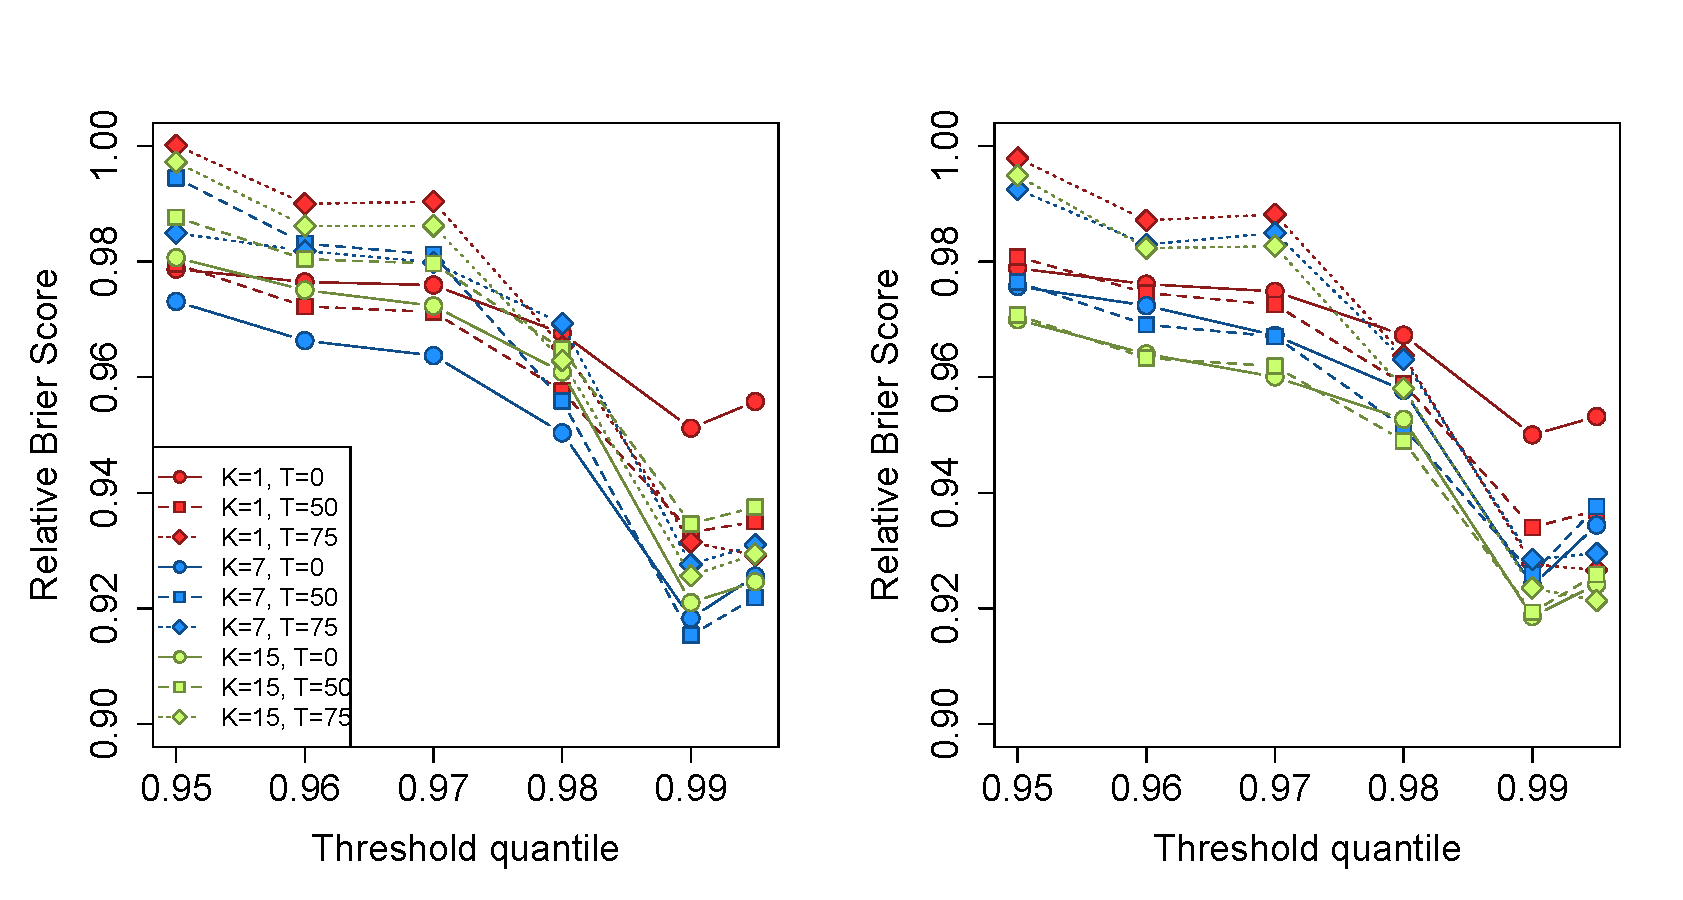
\includegraphics[width=\linewidth]{plots/bs-ozone.pdf}
  \caption{Relative Brier scores for time-series models (left) and non-time-series models (right). Relative brier score for the max-stable model is between 1.07 and 1.15}
  \label{fig:bs-ozone}
\end{figure}
\begin{table}
  \small
  \caption{Top two performing models for ozone analysis at extreme quantiles with Relative Brier score}
  \label{tbl:ozoneresults}
  \centering
  \begin{tabular}{|l|l l l c|l l l c|}
    \cline{2-9}
    \multicolumn{1}{c|}{}  & \multicolumn{4}{c|}{1st} & \multicolumn{4}{c|}{2nd} \\
    \hline
    $q(0.90)$  & No time series & $K=7$  & $T=0$  & BS: 0.980 &
                 No time series & $K=9$  & $T=0$  & BS: 0.980 \\
    $q(0.95)$  & No time series & $K=15$ & $T=50$ & BS: 0.970 &
                 No time series & $K=9$  & $T=50$ & BS: 0.970\\
    $q(0.98)$  & No time series & $K=5$  & $T=50$ & BS: 0.945 &
                 No time series & $K=10$ & $T=50$ & BS: 0.946\\
    $q(0.99)$  & Time series    & $K=10$ & $T=75$ & BS: 0.912 &
                 Time series    & $K=6$  & $T=75$ & BS: 0.913\\
    $q(0.995)$ & Time series    & $K=6$  & $T=75$ & BS: 0.917 &
                 Time series    & $K=10$ & $T=75$ & BS: 0.918\\
    \hline
  \end{tabular}
\end{table}

\begin{figure}
  \centering
  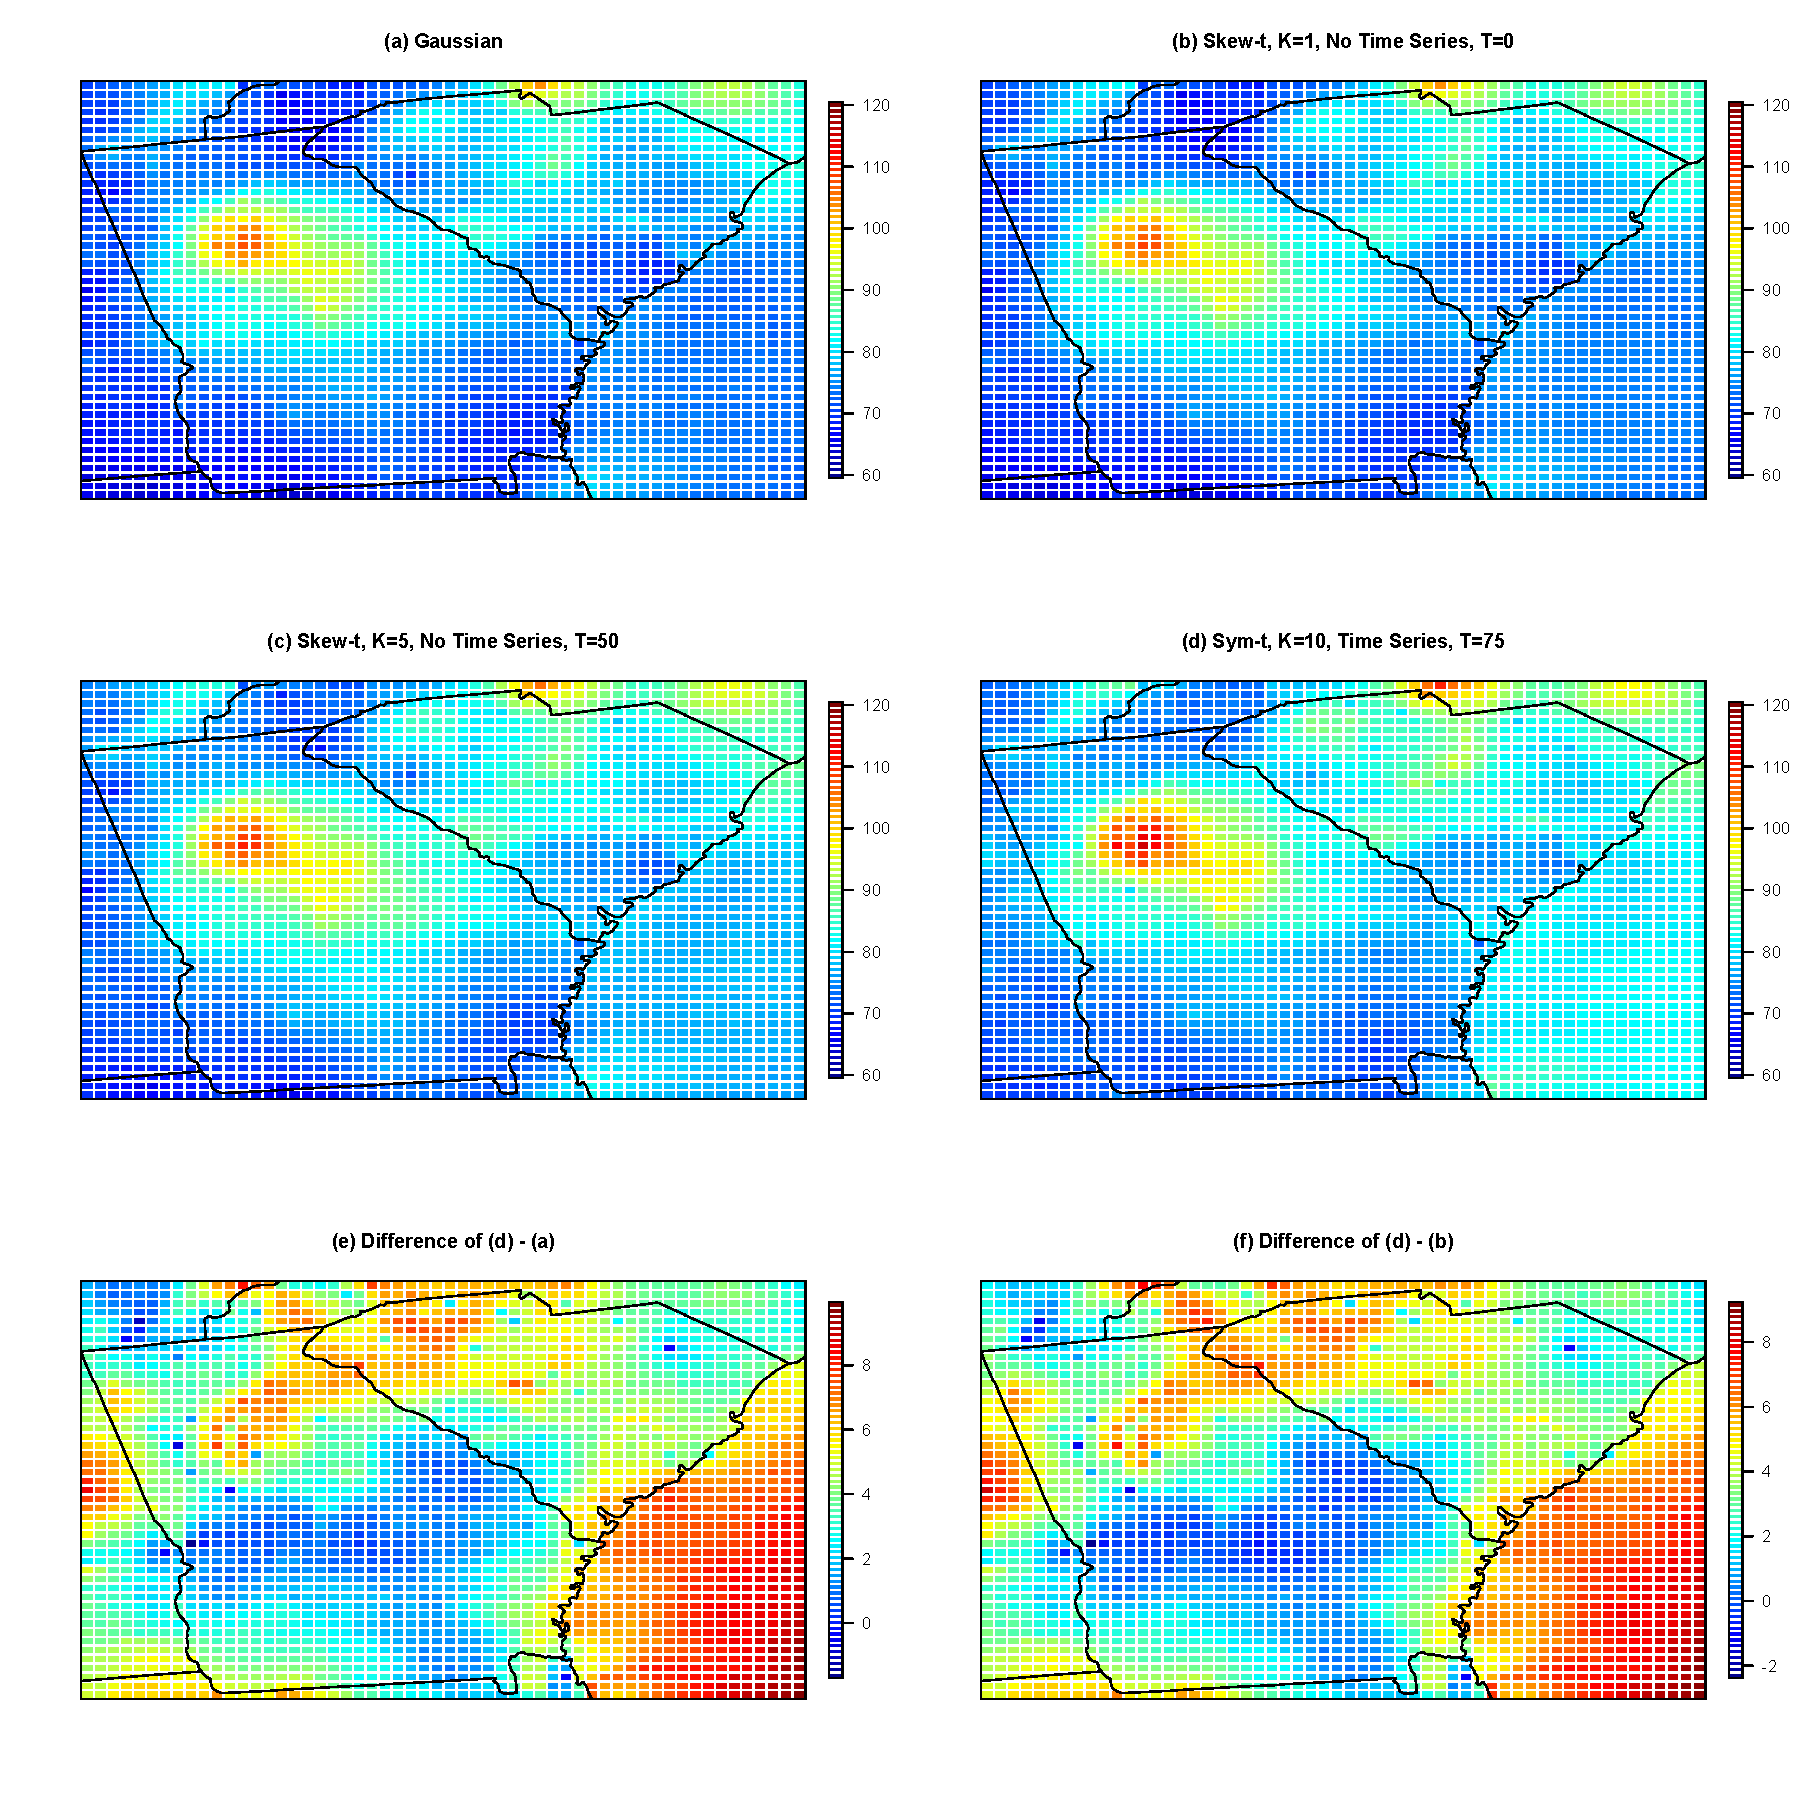
\includegraphics[width=0.8\linewidth]{plots/q99-ozone.pdf}
  \caption{Panels (a) -- (d) give the posterior predictive $\widehat{q}(0.99)$ for the month of July under four different models, panel (e) gives the difference between $\widehat{q}(0.99)$ in panels (d) and (a), panel (f) gives the difference between $\widehat{q}(0.99)$ in panels (d) and (b).}
  \label{fig:ozoneq99}
\end{figure}

\section{Discussion}\label{s:con}
In this paper we propose a new threshold exceedance approach for spatiotemporal modeling based on the skew-$t$ process.
The proposed model gives flexible tail behavior, demonstrates asymptotic dependence for observations at sites that are near to one another, and has computation on the order of Gaussian models for large space-time datasets.
In the simulation study, we demonstrate that this model shows statistically significant improvements over a na\"{i}ve Gaussian approach and in most cases, a max-stable approach.
In both the simulation study, and the application to ozone data, we find that incorporating a partition in the model can improve extreme predictions.
Furthermore the results from the data analysis suggest that thresholding can improve performance when predicting in the extreme tails of the data.

This model presents new avenues for future research.
One possibility is the implementation of a different partition structure.
We choose to define the random effects for a site by using an indicator function based on closeness to a knot.
However, this indicator function could be replaced by kernel function that would allow for multiple knots to impact each site, with the weight of each knot to be determined by some characteristic such as distance.
Another area that should be explored is the temporal dependence in the model.
Instead of implementing a time series on the random effects, a three-dimensional covariance structure on the residuals could be implemented to address temporal dependence.
Finally, we acknowledge that by specifying the number of knots, we may be underestimating the uncertainty in the model.
This could be incorporated by treating the number of knots as a model parameter instead of fixing it to be a specific value.

\backmatter

\section*{Acknowledgments}
The authors' work was partially supported by grants from the Department of the Interior (14-1-04-9), National Institutes of Health (R21ES022795-01A1), the US Environmental Protection Agency (R835228), the National Science Foundation (1107046), and the Research Network for Statistical Methods for Atmospheric and Oceanic Sciences (STATMOS).
The authors also received high-performance computing support from Yellowstone (ark:/85065/d7wd3xhc) provided by NCAR's Computational and Information Systems Laboratory, sponsored by the National Science Foundation.

\section*{Supplementary Materials}


\bibliographystyle{biom}
\bibliography{library}

\label{lastpage}

\end{document}

